%\documentclass[10pt,handout]{beamer}
\documentclass[10pt]{beamer}
\usepackage{babel} % Anpassa efter svenska. Ger svensk logga.
\usepackage[utf8]{inputenc} % Anpassa efter linux
\usepackage{graphicx}
\usepackage{../common/beamerthemeUppsala}
%\usetheme{Uppsala}
%\usecolortheme{UU} % Anpassa efter UU:s frger och logga
%\hypersetup{pdfpagemode=FullScreen} % Adobe Reader ska ppna fullskrm
\setbeamertemplate{itemize items}[circle]

% \usepackage{beamerthemesplit}
\usepackage{amsmath}
\usepackage{amssymb}
% \usepackage{graphics}
% \usepackage{graphicx}
% \usepackage{epsfig}
% \usepackage[latin1]{inputenc}
 \usepackage{color}
% \usepackage{fancybox}
% \usepackage{psfrag}
% \usepackage[english]{babel}
 \setbeamertemplate{footline}{\hfill\insertframenumber/\inserttotalframenumber}


% Read in commands
% Course settings
\newcommand{\currentsemester}{Autumn 2024}

% New commands
\newcommand{\bfm}[1]   {\mbox{\boldmath{${#1}$}}}
\newcommand{\Prob}   {\mbox{\textnormal{P}}}
\newcommand{\uured}[1]{\textcolor{uured}{#1}}

% Eqds
\def\eqd{\,{\buildrel d \over =}\,}

% Math operators
\DeclareMathOperator{\E}{\mathbb{E}}
\DeclareMathOperator{\V}{\mathbb{V}}


%%%%%%%%%%%%%%%%%%%%%%%%%%%%%%%%%%%%%%%%%%%%%%%%%%%%%%%%%%%%%%%%%%

\setlength{\parskip}{3mm}
\title[]{{\color{black}Machine learning -- Block 2}}
\author[]{M{\aa}ns Magnusson\\Department of Statistics, Uppsala University}
\date{\currentsemester}


\begin{document}

\frame{\titlepage
% \thispagestyle{empty}
}

%%%%%%%%%%%%%%%%%%%%%%%%%%%%%%%%%%%%%%%%%%%%%%%%%%%%%%%%%%%%%%%%%%


\begin{frame}{This week's lecture}
\begin{itemize}
\item Trees
\item Bagging
\item Random Forest
\item Boosting (Trees)
\end{itemize}
\end{frame}



%%%%%%%%%%%%%%%%%%%%%%%%%%%%%%%%%%%%%%%%%%%%%%%%%%%%%%%%%%%%%%%%%%

\frame{\frametitle{Assignment 1}


\begin{enumerate}
\item Assignment 1: Overall satisfaction
\end{enumerate}

}


\section{Decision trees}
\frame{\sectionpage}

\frame{\frametitle{Decision trees: basic idea}
\begin{itemize}
\item A popular method that can be used for both classification and regression is \uured{decision trees}.\pause
\item Have you ever played the game ''20 questions''?\\[3mm]\pause
\item Decision trees is more or less that game!\\[3mm]\pause
\item In the case of classification, the idea is to classify the new observation by
\begin{enumerate}
\item Asking a questions
\item Based on the previous answer, ask new question
\item Questions are asked until a conclusion is reached
\end{enumerate}
\end{itemize}
}

\frame{\frametitle{Decision trees: basic idea}
{\small
\begin{table}[ht]
\begin{tabular}{l| l|l|l|l}
{\bf Name} & {\bf Body temp}& {\bf Gives birth}& {\bf Legs}& {\bf Class} \\
\hline
Human & warm-blooded & yes & yes & mammal\\
Whale & warm-blooded & yes & no & mammal\\
Cat & warm-blooded & yes & yes & mammal\\
Cow & warm-blooded & yes & yes & mammal\\\hline
Python & cold-blooded & no & no & reptile\\
Komodo dragon & cold-blooded & no & yes & reptile\\
Turtle & cold-blooded & no & yes & reptile\\\hline
Salmon & cold-blooded & no & no & fish\\
Eel & cold-blooded & no & no & fish\\\hline
Pigeon & warm-blooded & no & yes & bird\\
Penguin & warm-blooded & no & yes & bird
\end{tabular}
\end{table}}
\pause
Classify \uured{Komodo dragon} with a decision tree:
\begin{enumerate}
\item Does it give live birth? \pause (\uured{No!})
\item Is it warm-blooded? \pause (\uured{No!})
\item Does it have legs? \pause (\uured{Yes!}) $\rightarrow$ \uured{Reptile}
\end{enumerate}

}


\frame{\frametitle{Regression trees: The regions of a tree}

\begin{figure}[h]
\centering
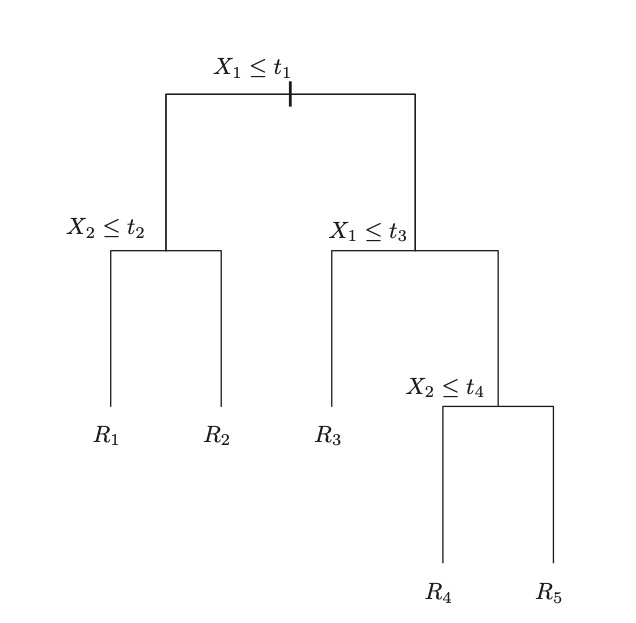
\includegraphics[width=0.45\textwidth]{fig/ISL_8_3_b.png}
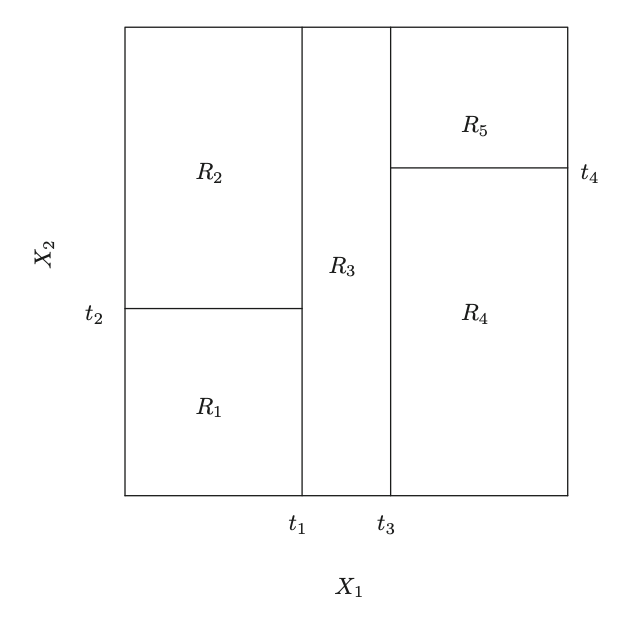
\includegraphics[width=0.45\textwidth]{fig/ISL_8_3_a.png}
\caption{Regions of a tree (Garreth et al, 2013, Fig. 8.3)}
\end{figure}

}



\frame{\frametitle{Regression Trees}

\[
T(x) = \sum^M_{m=1} \gamma_m I(x \in R_m)\,,
\]
where $M$ is the total number of regions and $I(x \in R_m)$ is an indicator variable if $x_i$ belongs to region $R_m$ and $\gamma_m$ is the prediction for region $m$.

}

\frame{\frametitle{Regression Trees}

\begin{figure}[h]
\centering
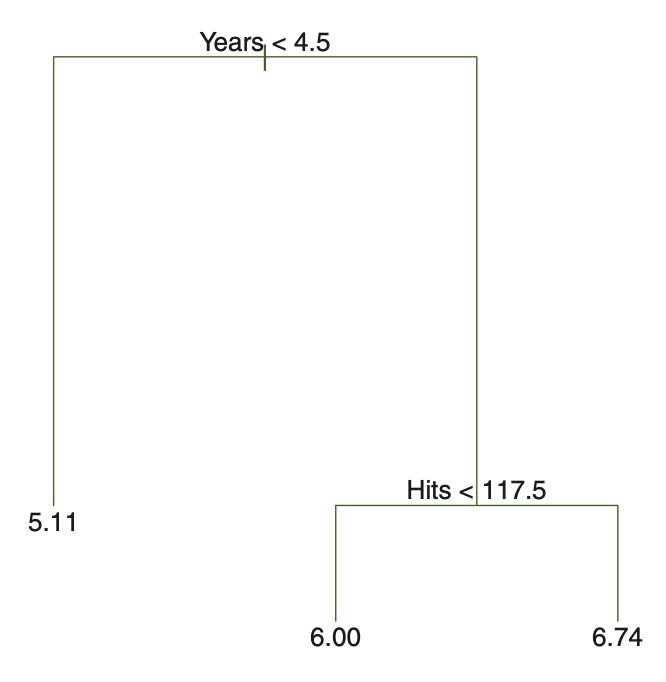
\includegraphics[width=0.5\textwidth]{fig/ISL_8_1_tree.png}
\caption{Regression Tree (Garreth et al, 2013, Fig. 8.1.)}
\end{figure}

\begin{itemize}
\item The \texttt{Hitters dataset}: log Salaries of Baseball players.
\item The end of the tree contain the observations.
\end{itemize}
}



\frame{\frametitle{Regression Trees}

\begin{figure}[h]
\centering
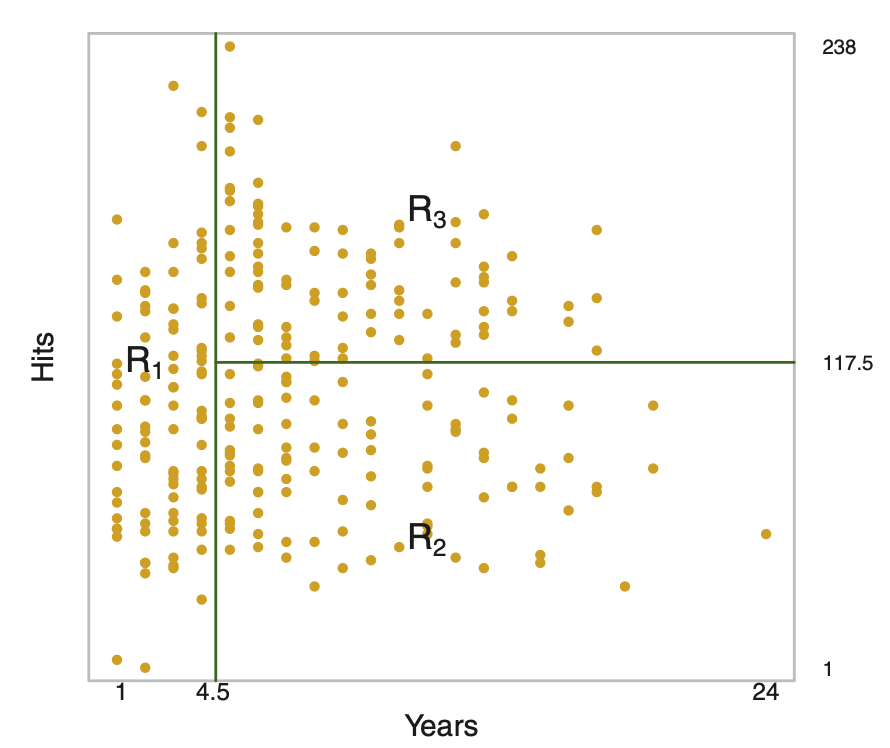
\includegraphics[width=0.8\textwidth]{fig/ISL_8_2_tree.png}
\caption{\texttt{Hitters} data and regression tree regions (Garreth et al, 2013, Fig. 8.2.)}
\end{figure}

}


\frame{\frametitle{Estimating a Decision Tree}

\begin{enumerate}
\item A tree has two groups of parameters $\Theta = (\gamma, R)$ that we need to learn.\pause
\item We want a tree that minimize $L(\theta) = \sum_i^N (y_i - T_\Theta(x_i))^2$, here the squared loss\pause
\item Usually we estimate $\gamma_m$ as the mean of $y_i$ in the region as:
\[
\hat{\gamma}_m = \frac{1}{N_m} \sum_{x_i \in R_m}^{N_m} y_i\,,
\]
where $N_m$ is the number of observations in region $R_m$.\pause
\item Learning $R_m$ exact is generally computationally infeasable so we use a \uured{greedy} heuristic.
\end{enumerate}

}



\frame{\frametitle{Growing a Decision Tree: Greedy Algorithm}


Let $\mathcal{S}$ be the set of all observations $\{1,...,N\}$ and \texttt{S[[m]]} be the set of observation indecies in $R_m$ and \texttt{l} is the minimal number of leafs per node.

Input: $\mathcal{S}, \texttt{X}, \texttt{y}, \texttt{l}$

\begin{enumerate}
\item \texttt{S[[1]]} = $\mathcal{S}$,\texttt{M = 1}, \texttt{m = 1}
\item \texttt{while m <= M} then do:
\begin{enumerate}
\item \texttt{if(size(S[[m]]) >= 2*l)}
\begin{enumerate}
\item \texttt{S[[M+1]]}, \texttt{S[[M+2]]}, \texttt{j[m]}, \texttt{s[m]} = \\ \texttt{split\_tree(X[S[[m]],], y[S[[m]],],l)}
\item \texttt{M = M + 2}
\end{enumerate}
\item \texttt{else}
\begin{enumerate}
\item compute $\hat{\gamma}$ for \texttt{S[[m]]}
\end{enumerate}
\item \texttt{m = m + 1}
\end{enumerate}
\end{enumerate}

Output: $\texttt{j}, \texttt{s}, \gamma$

Example of a tree:
\texttt{j = \{Years, Hits\}}, \texttt{s = \{4.5, 117.5\}}, $\hat{\gamma} = \{122, 317, 245\}$

}

\frame{\frametitle{How to do a split?}

Here we try to compute Eq. (9.12-9.14) in ESL:

\[
R_1(j,s) = \{X|X_j\leq s \}\text{ and } R_2(j,s) = \{X|X_j > s \}
\]

\[
\min_{j,s} \left(\min_{c_1} \sum_{x_i \in R_1(j,s)} (y_i - c_1)^2 + \min_{c_2} \sum_{x_i \in R_2(j,s)} (y_i - c_2)^2\right)
\]

Inner minimization is solved by:
\[
\hat{c}_m = \frac{1}{N_m} \sum_{x_i \in R_m}^{N_m} y_i\,,
\]

}

\frame{\frametitle{How to do a split? Pseudo-code}



Input: $\mathbf{X}, \mathbf{y}, l$

\begin{enumerate}
\item $SS$ = Inf \# Store sum of squares in matrix of dim $P\times N_s$
\item $S$ = Inf \# Store split point in matrix of dim $P\times N_s$
\item for $j \in \{1,...,P\}$ \# all features
\begin{enumerate}
\item for $k \in \{1,...,N_s\}$ \# all observations in set $s$
\begin{enumerate}
\item $s$ = $x_{k,j}$ \# Split point (use the value of x)
\item if ($|R_1(s, j)| < l$ or $|R_2(s, j)| < l$) next \# Dont create too few leaves
\item $\hat{c}_1$ = $\frac{1}{|R_1(s, j)|} \sum_{x_i \in R_1(s, j)} y_i$
\item $\hat{c}_2$ = $\frac{1}{|R_2(s, j)|} \sum_{x_i \in R_2(s, j)} y_i$
\item $SS_{k,j}$ = $\sum_{x_i \in R_1(s, j)} (y_i - c_1)^2 + \sum_{x_i \in R_2(s, j)} (y_i - c_2)^2$ \# Compute Sum of Squares
\item $S_{k,j}$ = s
\end{enumerate}
\end{enumerate}
\item $k_{final}, j_{final} = \min_{k,j} SS$
\item $s_{final} = S_{k_{final},j_{final}}$
\item return $R_1(s_{final}, j_{final}), R_2(s_{final}, j_{final}), s_{final}, j_{final}$
\end{enumerate}
}



\frame{\frametitle{Decision trees: Classification Trees}

\begin{itemize}
\item \uured{How do we do if we have a classification tree?}\pause
\item We just change the loss function $L(\theta)$.\pause
\item Let $p(j|t)$ be the fraction of observations in class $j$ at the node $t$ and let $J$ be the number of classes.\pause
\item The {\color{uured}Gini} for node $t$ is defined as
\[
Gini(t)=1-\sum_{j=1}^J p(j|t)^2
\]\pause
\item Gini is a measure of ''impurity''. If all observations belong to the same class, then
\[
Gini(t)=1-1^2-0-\ldots-0=0.
\]\pause
\item The Gini is maximized when all classes have the same number of observations at $t$.\\[2mm]\pause
\item One criterion for splitting could be to minimize the Gini in the next level of the tree. That way we will get ''purer'' nodes.
\end{itemize}





}


%\frame{\frametitle{Decision trees: the best split}
%The situation becomes a bit more complicated if we take into account that the children can have different numbers of observations. \pause To account for this, we try to maximize the gain:
%\[
%Gain=Gini(t)-\sum_{j=1}^k \frac{n_{v_j}}{n_t}Gini(v_j)
%\]
%where $v_j$ are the children and $n_i$ are the number of observations at node $i$.\\[2mm]\pause
%This is equivalent to minimizing $\sum_{j=1}^k \frac{n_{v_j}}{n_t}Gini(v_j).$\\[2mm]\pause
%Sometimes other impurity measures than Gini are used. One example is the {\color{uured}entropy}:
%\[
%Entropy(t)=-\sum_{i=1}^cp(i|t)\log_2p(i|t).
%\]
%}

\frame{\frametitle{Important concepts in trees}
\begin{itemize}
\item {\color{uured}Tree depth:} the length of the longest path from the root to a leaf (i.e. greatest number of questions that the tree can ask).\\[2mm]\pause
\item {\color{uured}Leaf size:} the number of observations in a leaf.\\[2mm]\pause
\end{itemize}
Decision trees can become quite large, which may lead to:
\begin{itemize}
\item Overfitting (high variance)
\item Difficulties interpreting the tree\\[2mm]\pause
\end{itemize}
The solution to this is
\begin{itemize}
\item {\color{uured}Pruning:} forcing the tree to be smaller by adding a {\color{uured}stopping condition}, e.g. a maximum depth or minimal leaf size.\pause
\item But decision trees are quite bad predition models...
\end{itemize}
}

%%%%%%%%%%%%%%%%%%%%%%%%%%%%%%%%%%%%%%%%%%%%%%%%%%%%%%%%%%%%%%%%%%

\section{Ensemble methods}
\frame{\sectionpage}

\frame{
\frametitle{Wisdom of the crowd}

Simulated example (Prize academy, see ESL):
\begin{enumerate}
\item 50 members vote in 10 categories, each with 4 nominations.
\pause
\item For any category, only 15 voters have some knowledge ($p>0.25$)
\pause
\item For each category, the 15 experts are chosen at random from the 50.
\end{enumerate}
}


\frame{
\frametitle{Wisdom of the crowd}

\begin{figure}[h]
\centering
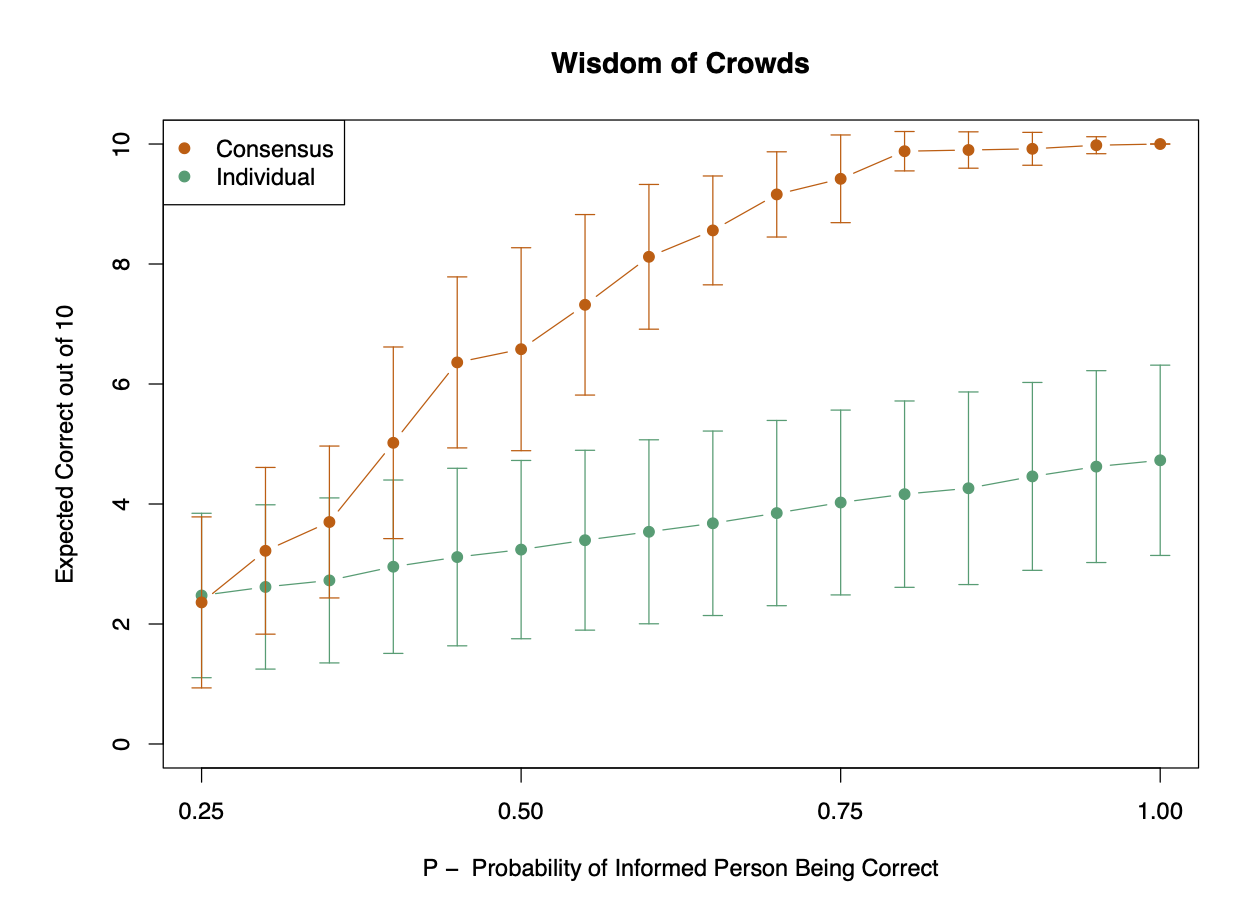
\includegraphics[width=0.99\textwidth]{fig/wisdom_esl8_11}
\caption{Simulated Award Voting, Fig. 8.11 (ESL)}
\end{figure}
%If the 15 informed for a category have a 50\% chance of selecting the correct candidate, the consensus doubles the expected performance of an individual.
}



\frame{\frametitle{General idea of ensembles}
The idea of an ensemble is simple: If it difficult to find one really good model perhaps we can find \uured{several weaker models} and \uured{combine their predictions}.\\~\\ \pause
%
\uured{A simple example}: Say you have one outcome $Y$ and 4 covariates $X_1,X_2,X_3,X_4$. The goal is to predict $Y$. A possible ensemble would be to fit
\begin{align*}
y=\alpha_1 + \beta_1X_1 + \epsilon_1\\
y=\alpha_2 + \beta_2X_2 + \epsilon_2\\
y=\alpha_3 + \beta_3X_3 + \epsilon_3\\
y=\alpha_4 + \beta_4X_4 + \epsilon_4
\end{align*}
and then use the mean of their predictions
\begin{equation}
\hat{y}_{ensemble}=\frac{1}{4}\sum_{i=1}^4 \hat{y}=\frac{1}{4}\sum_{i=1}^4(\hat{\alpha}_i + \hat{\beta}_iX_i)
\end{equation}

}

%
%
%

\frame{\frametitle{Two key parts of an ensemble}
\begin{enumerate}
\item \uured{The prediction models} (sometimes called `learners')
\begin{itemize}
\item A single model in an ensemble can be a simple or a complex model
\item Often the ensemble contains many simple models.
%\item Wikipedia:``\textit{In statistics and machine learning, ensemble methods use multiple learning algorithms to obtain better predictive performance than could be obtained from any of the constituent learning algorithms alone}''
\end{itemize}
\pause
\item \uured{The weighting of each prediction} in the final ensemble prediction
\begin{itemize}
\item Many different algorithms for weighting together the predictions from many models
\item Models/learners with better predictive power can be given larger weights in the final prediction
\end{itemize}
\end{enumerate}
}



\frame{\frametitle{Ensambles of decision trees}
\begin{itemize}
\item A common type of ensembles is ensembles of decision trees.
\item We will focus on this case, \uured{but note that any type of model can be included in an ensemble} in principle.\\~\\
\end{itemize}
}
%%%%%%%%%%%%%%%%%%%%%%%%%%%%%%%%%%%%%%%%%%%%%%%%%%%%%%%%%%%%%%%%%%



%\section{Bagging and Boosting}
\frame{\frametitle{Bagging and Boosting}

Remember, the error of a prediction/classification can be decomposed as
\begin{equation}
error = bias^2 + variance + bayes error.
\end{equation}
\pause
\begin{itemize}
\item \uured{Complex models/strong learners} (with many parameters) tend to have small bias and large variance (tend to be overfitted)\pause
\item \uured{Shallow models/weak learners} (with few parameters) tend to have small variance and large bias
\end{itemize}
\pause


\uured{Bagging:} Ensemble methods that aim to decrease the variance of complex/strong learners with low bias and large variance\\~\\
\uured{Boosting:} Ensemble methods that aim to decrease the bias of shallow/weak learners with low variance and large bias

%That is: Either choose models with small bias and reduce the variance with bagging, or choose models with small variance and reduce bias with boosting
}


\subsection{Bagging}
\frame{\subsectionpage}


\frame{\frametitle{Bagging (Bootstrap AGGregating)}

\begin{itemize}
\item Train several \uured{deep} trees and combine their results
\item Use bootstrap to train different trees
\end{itemize}

\begin{figure}[h]
\centering
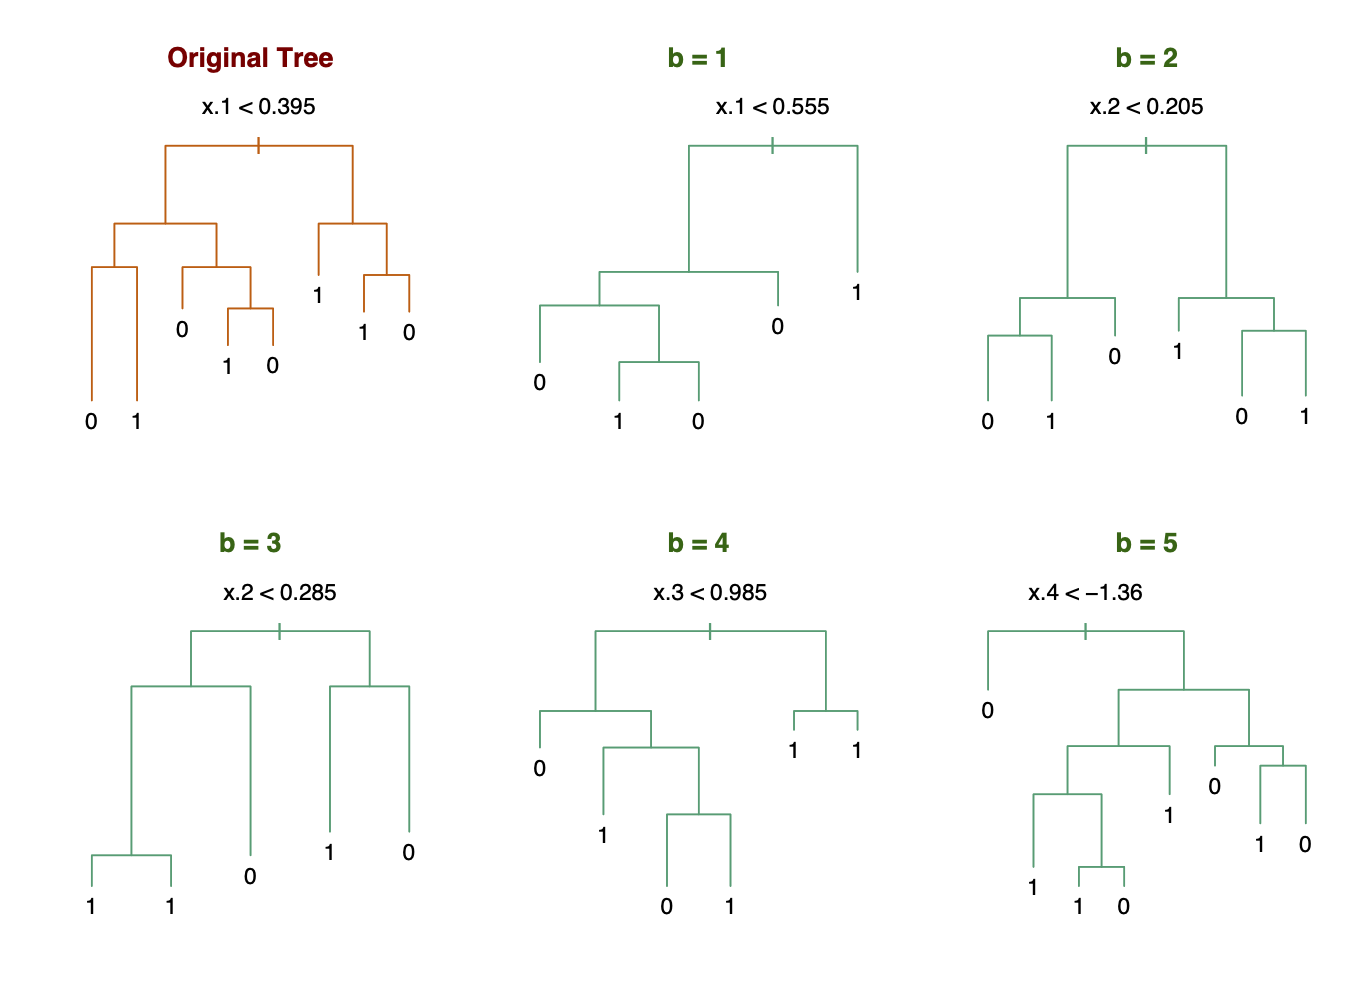
\includegraphics[width=0.9\textwidth]{fig/bagging_esl_8_9}
\caption{Bagging trees, Fig. 8.9 (ESL)}
\end{figure}


}

\frame{\frametitle{Bagging (Bootstrap AGGregating)}

\begin{enumerate}
\item Draw, \textit{with replacement}, a random sample of $N$ units from the original sample
\item Fit a prediction model (e.g., a \uured{deep} decision tree)
\item Repeat steps 1-2 $B$ times
\item Weight together the predictions from the B models into a final ensemble prediction as
\[
\hat{f}_\text{bag}(x_i)=\frac{1}{B}\sum_b \hat{f}^b (x_i) = \frac{1}{B}\sum_b \hat{T} (x_i | \Theta_b)
\]
\end{enumerate}


}







%%%%%%%%%%%%%%%%%%%%%%%%%%%%%%%%%%%%%%%%%%%%%%%%%%%%%%%%%%%%%%%%%%

\subsection{Random forests}
\frame{\subsectionpage}

\frame{\frametitle{Random Forest}

\begin{itemize}
\item A bagging ensemble method, but...
\pause
\item Sample of $N$ observations and $K$ covariates/features
\pause
\item It is common to use $k=\sqrt{K}$ (rounded down) for classification and $k=K/3$ for regression. But these are only rules of thumb: $k$ is a \textit{tuning parameter}.
\end{itemize}
}



\frame{\frametitle{Random Forest: Algorithm}

\begin{enumerate}
\item Draw, \textit{with replacement}, a random sample of $N$ units from the original sample
\item \textbf{Draw,  \textit{without replacement}, a random subset of $k$ covariates/features}
\item Fit a prediction model (e.g., a decision tree)
\item Repeat step 1-3 $B$ times
\item Weight together the predictions from the B models into a final ensemble prediction
\[
\hat{f}_\text{rf}(x_i) = \frac{1}{B}\sum_b \hat{T} (x_i | \Theta_b)
\]
\end{enumerate}


}

\frame{\frametitle{Random Forest variance reduction}
\begin{itemize}
\item Consider each tree to be an i.i.d. random variable with variance $\sigma^2$.
\item The average of these trees then have variance
\begin{align*}
\V (\hat{f}(x) = \frac{1}{B}\sigma^2.
\end{align*}
	\pause
\item Trees constructed from the same set of covariates will be correlated and therefore \uured{not independent}.
\item The variance of the average of these correlated trees then becomes
	\begin{align*}
	\V (\hat{f}(x)) = \rho\sigma^2+\dfrac{1-\rho}{B}\sigma^2.
	\end{align*}
\end{itemize}

}

\frame{\frametitle{Random Forest variance reduction}
\begin{itemize}
\item The variance of the average of correlated trees:
	\begin{align*}
	\V (\hat{f}(x)) = \rho\sigma^2+\dfrac{1-\rho}{B}\sigma^2.
	\end{align*}
	\item The second term will \uured{vanish with increasing $B$} leaving just the first term left: a function of the \uured{correlation between the trees}
	\pause
	\item The remaining part of the variance is minimized by only consider a subset of the covariates when constructing trees - \uured{reducing the correlation} between trees.
\end{itemize}

}

\frame{
\frametitle{Bagging vs. Random forest}
\begin{itemize}
\item In bagging, the trees are often highly correlated
\begin{itemize}
\item If some covariates are strong predictors of the outcome (in the training data), many trees in the `bag' will us the same covariates in their decisions
\end{itemize}
\pause
\item In a random forest, the trees are less similar/correlated since all covariates are not available when each tree is constructed.
\pause
\item Intuition: A random forest (with many trees) uses the predictive ability of all covariates rather than just a few $\rightarrow$ improved out of sample performance.
\end{itemize}
}




%%%%%%%%%%%%%%%%%%%%%%%%%%%%%%%%%%%%%%%%%%%%%%%%%%%%%%%%%%%%%%%%%%

\subsection{(Gradient) Boosting}
\frame{\subsectionpage}

\frame{\frametitle{Boosting}

\begin{enumerate}
\item In boosting, models/trees are trained \uured{sequentially}
\pause
\item Each new model tries to target \uured{weak spots of the previous models}
\end{enumerate}

}


\frame{\frametitle{Boosting (AdaBoost)}

\begin{enumerate}
\item Initialize weight for all observations as $w_i = n^{-1}$
\item Repeat $B$ times
\begin{enumerate}
\item Fit a simple classifier $h_b(x)$ using $w_i$s
\item Compute the weighted error (between 0-1) as
\[
e_b = \frac{\sum w_i I(y_i \neq h_b(x_i))}{\sum w_i}
\]
\item Compute the importance of the classifier as
\[
\alpha_b = \log((1-e_b)/e_b) = \text{logit}(1-e_b)
\]
\item Add the classifier to the ensemble
\[
\hat{f}_b(x) = \hat{f}_{b-1}(x) + \alpha_b h_b(x)
\]
\item Update weights so that badly classified observations is weighted more
\[
w_i \leftarrow w_i \exp (\alpha_b I(y_i \neq h_b(x_i)) )
\]
\end{enumerate}
\item Output the final ensemble $\hat{f}_B(x)$
\end{enumerate}

}

\frame{\frametitle{Boosting example}

\begin{figure}[h]
\centering
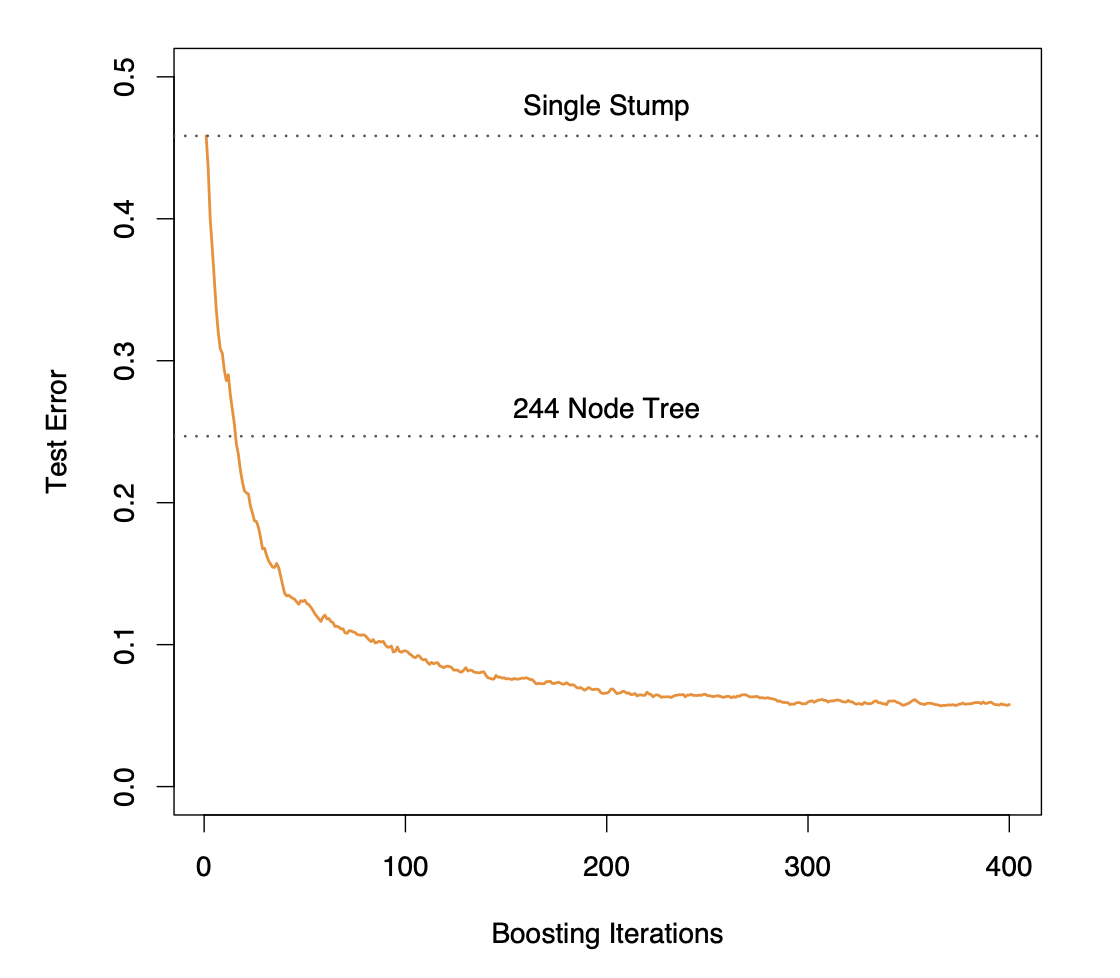
\includegraphics[width=0.9\textwidth]{fig/esl_10_2_adaboost}
\caption{Boosting example (using stumps as $h_b$), Fig. 10.2 (ESL)}
\end{figure}

}


\frame{\frametitle{Boosting trees}

\begin{itemize}
\item A more general approach is \uured{(gradient) boosting trees}
\pause
\item Let
\[
f_\text{gb}(x) = \sum^B_b \hat{T} (x | \Theta_b)
\]
\pause
\item We want to minimize the loss
\[
L(y, f_\text{gb}(x))
\]
\pause
\item This means finding
\[
\Theta_b = \arg \min \sum^N_i L(y_i, f_{b-1}(x_i) + \hat{T} (x | \Theta_b))
\]
\end{itemize}

}


\frame{\frametitle{Gradient Boosting Trees}

\begin{enumerate}
\item Initialize $f_{0}(x)$
\item Repeat $B$ times
\begin{enumerate}
\item For $i=1,2,...,N$ compute
\[
r_{ib} = - \frac{\partial L(y_i,f(x_i))}{\partial f(x_i)}
\]
\item Compute a regression tree $\hat{T} (x | \Theta_b)$ on $r_b$
\item Add the classifier to the ensemble
\[
\hat{f}_b(x) = \hat{f}_{b-1}(x) + \hat{T} (x | \Theta_b)
\]
\end{enumerate}
\item Output the final ensemble $\hat{f}_B(x)$
\end{enumerate}

}

\frame{\frametitle{Comparisons}

\begin{figure}[h]
\centering
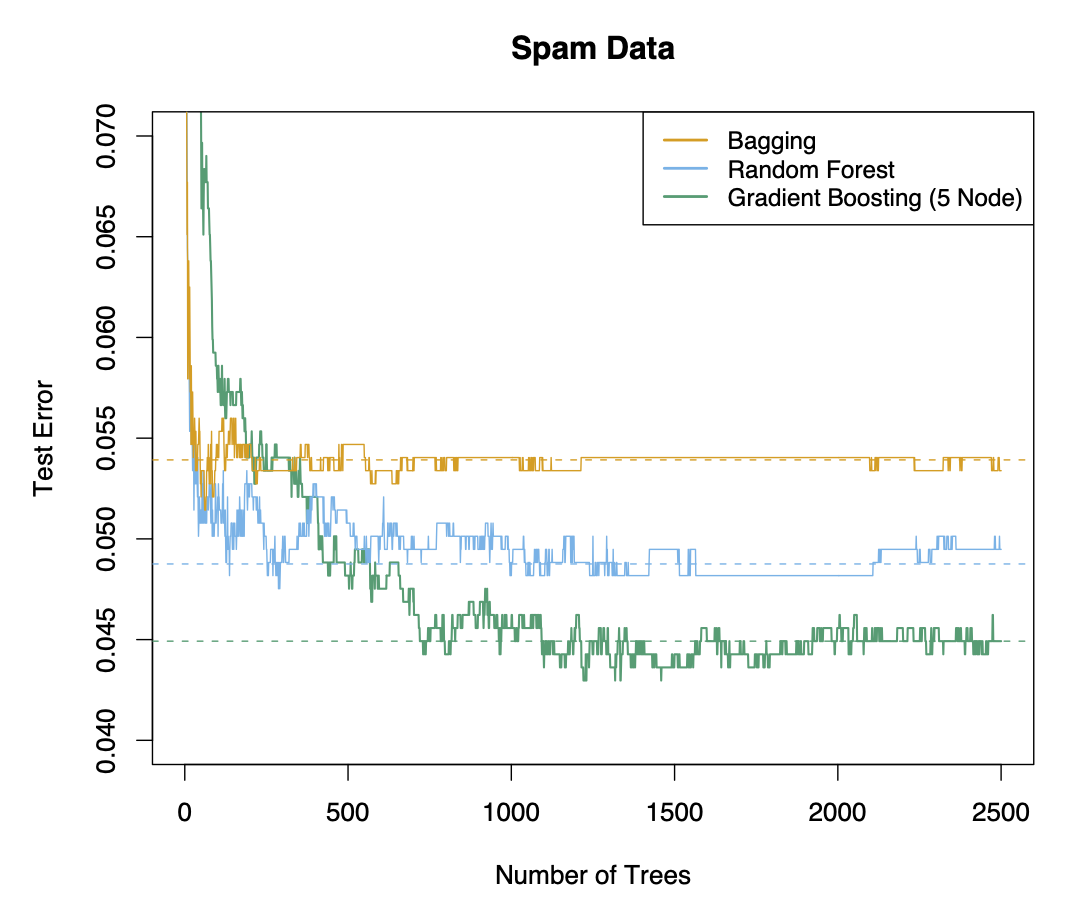
\includegraphics[width=0.9\textwidth]{fig/esl_15_1_compare}
\caption{Comparing bagging, random forests and boosting, Fig. 15.1 (ESL)}
\end{figure}

}


\frame{\frametitle{XGBoost}

\begin{itemize}

\item State of the Art method\pause
\item Use gradient boosting trees with regularization
\[
L(y, f_\text{boost}(x)) + \sum_b \Omega(\hat{T} (x_i | \Theta_b))
\]
\pause
where
\[
\Omega(\hat{T} (x_i | \Theta_b)) = \lambda_1 Q_b + \lambda_2 ||\gamma_b||_2^2
\]
where $Q_b$ is the number of leafs in tree $b$ and $||\cdot||_2$ is the Euclidian/$L^2$ norm.
\pause
\item Is scalable to very large data
\end{itemize}

}



\end{document}
